\documentclass[11pt]{article}
\usepackage[margin=1in]{geometry}
\usepackage[T1]{fontenc}
\usepackage[utf8]{inputenc}
\usepackage{amsmath,amssymb}
\usepackage{booktabs,array,longtable}
\usepackage{graphicx}
\usepackage{float}
\usepackage{xcolor}
\usepackage{hyperref}
\usepackage{enumitem}
\hypersetup{colorlinks=true, linkcolor=blue!60!black, urlcolor=blue!60!black, citecolor=blue!60!black}
\setlength{\parindent}{0pt}
\setlength{\parskip}{0.55em}
\setlist[itemize]{leftmargin=1.25em,itemsep=0.2em,topsep=0.25em}
\setlist[enumerate]{leftmargin=1.45em,itemsep=0.2em,topsep=0.25em}

\newcommand{\statusbox}[2]{%
  \noindent\fcolorbox{black}{gray!10}{%
    \parbox{\dimexpr\linewidth-2\fboxsep-2\fboxrule\relax}{%
      \textbf{Status:} #1\\#2
    }%
  }
}
\newcommand{\Jphys}{J_{\mathrm{phys}}}
\newcommand{\Jlin}{J_{\mathrm{lin}}}
\newcommand{\Jsurf}{J_{\mathrm{surf}}}
\newcommand{\band}{\mathcal{B}_{\mathrm{Raman}}}
\newcommand{\uhat}{\hat{u}}
\newcommand{\utilde}{\tilde{u}}
\newcommand{\Nt}{N_t}
\newcommand{\Omegaoff}{\Omega}

\title{Current Equation Verification for the Raman-Suppression Codebase}
\author{Fiber Raman Suppression Project}
\date{Evidence snapshot: 2026-04-26}

\begin{document}
\maketitle

\begin{abstract}
This document is the current verification backbone for the research-note
series. It checks the equations that matter most for the active codebase:
the interaction-picture forward model, Raman-band objective, adjoint phase
gradient, regularized dB objective, reduced-basis chain rule, Hessian and
trust-region interpretation, multimode gradients, and multivariable
chain-rule paths. The goal is not to replace every research note with one huge
derivation. The goal is to give each note a compact, auditable place to point
when a reader asks, ``Where did this equation come from, where is it in code,
and how was it checked?'' Some items are verified by existing tests and saved
artifacts. A few heavyweight reruns are still pending and are explicitly marked
as such.
\end{abstract}

\section*{Claim Status}
\statusbox{current verification map; burst reruns pending}{The derivations and
source-path audit below reflect the current codebase as of 2026-04-26. The
single-mode phase-gradient path, regularized objective convention, reduced-basis
chain rule, finite-difference HVP interpretation, and MMF mode-coordinate
finite-difference policy are ready to cite with the caveats shown. The full
production verification suite and the multivariable gradient smoke suite still
need fresh burst reruns before the whole note series should be called
publication-grade.}

\section{How To Read This Document}

Each equation is checked through the same stack:

\begin{figure}[H]
\centering
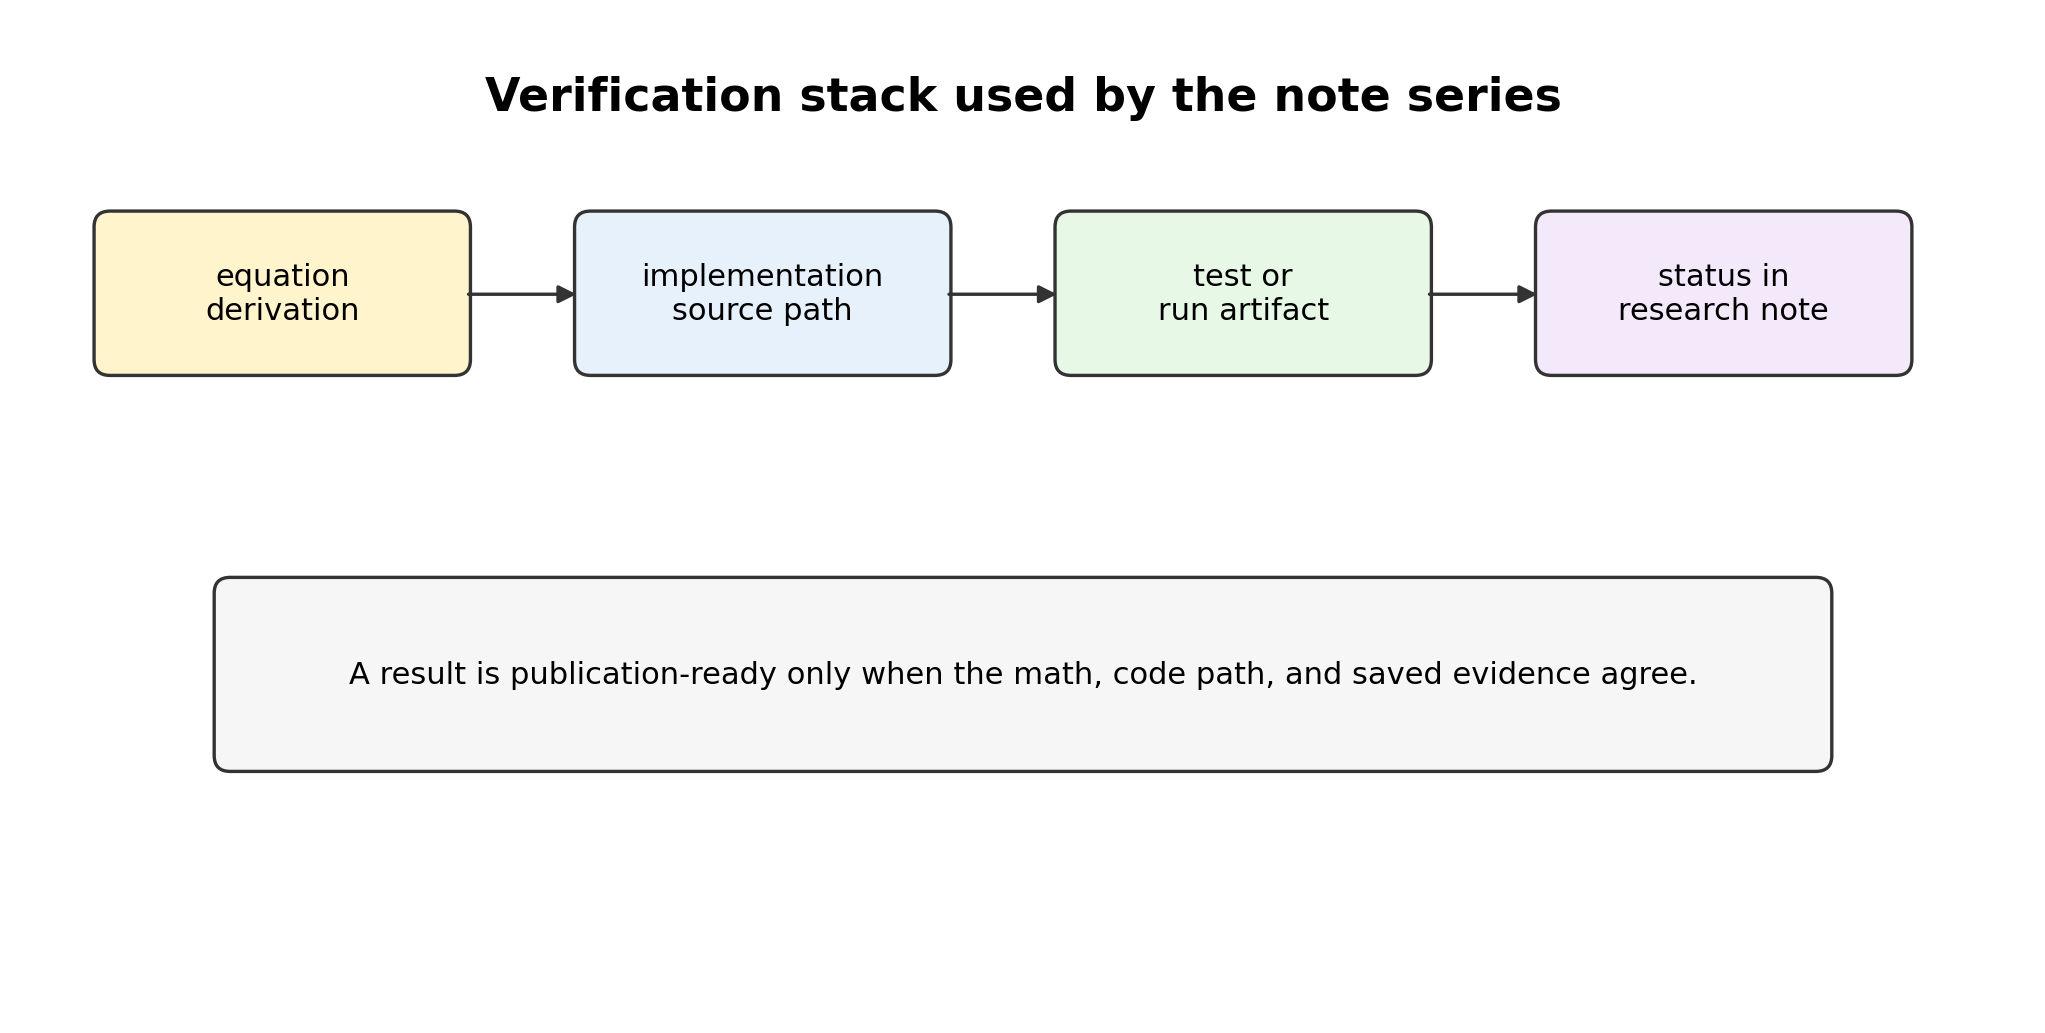
\includegraphics[width=0.92\linewidth]{figures/verification_stack.png}
\caption{Verification stack. A mathematical claim is only useful for the note
series when the derivation, source path, and test or run artifact all agree.}
\end{figure}

\textbf{Verified} means the equation is implemented and has an appropriate
finite-difference, Taylor, identity, or regression check.

\textbf{Verified with caveat} means the main equation is usable, but the note
must state an important scope limit.

\textbf{Finite-difference by design} means the project intentionally does not
claim an analytic derivative for that block.

\textbf{Pending rerun} means the code path has evidence, but a current
publication-grade run has not yet been refreshed.

\subsection*{Intuition Check}

The point is not to make every reader redo all the math. The point is to make
the logic traceable: equation, code, check, and conclusion.

\section{Forward Fiber Model}

The propagated spectral field in the lab frame is \(\uhat(z,\omega)\). Here
\(\omega\) denotes the absolute angular-frequency grid used by the code. If a
derivation instead uses the offset \(\Omegaoff=\omega-\omega_0\), the
self-steepening factor below is \(1+\Omegaoff/\omega_0\). The
generalized nonlinear Schrodinger equation used by the project is the standard
nonlinear-fiber model with dispersion, Kerr nonlinearity, delayed Raman
response, and self-steepening \cite{agrawal2019,hult2007}. In compact form:
\[
    \frac{\partial \uhat}{\partial z}
    =
    iD(\omega)\uhat
    +
    i\frac{\omega}{\omega_0}
    \mathcal{F}\!\left[
      \gamma(1-f_R)|u|^2u
      +\gamma f_R(h_R * |u|^2)u
    \right].
\]
The implementation stores the delayed Raman fraction inside the discrete
Raman-response array and stores the instantaneous fraction separately as
\(1-f_R\). This is algebraically the same convention as the equation above if
\(h_R\) is interpreted as a unit-normalized Raman response.

The code integrates the interaction-picture field
\[
    \utilde(z,\omega)=e^{-iD(\omega)z}\uhat(z,\omega).
\]
Differentiating gives
\[
    \frac{\partial \utilde}{\partial z}
    =
    i e^{-iD(\omega)z}
    \frac{\omega}{\omega_0}
    \mathcal{F}\!\left[
      \gamma(1-f_R)|u|^2u
      +\gamma f_R(h_R * |u|^2)u
    \right],
\]
where the nonlinear term is evaluated from the lab-frame field
\(\uhat=e^{iDz}\utilde\).

\textbf{Convention check.} With the code's interaction-picture definition,
the lab-frame linear term is \(+iD(\omega)\uhat\). Changing the Fourier sign
convention or redefining \(D\) can move the minus signs around, so verification
must compare the complete pair: transform convention plus dispersion
definition plus self-steepening factor.

\begin{center}
\small
\begin{tabular}{>{\raggedright\arraybackslash}p{0.30\linewidth}
                >{\raggedright\arraybackslash}p{0.58\linewidth}}
\toprule
\textbf{Implementation path} & \textbf{What to check} \\
\midrule
\shortstack[l]{\texttt{src/simulation/}\\
\texttt{simulate\_disp\_mmf.jl}} &
\texttt{disp\_mmf!} applies \(e^{iDz}\), transforms to time, builds Kerr and
Raman terms, applies self-steepening, and returns to the interaction picture. \\
\texttt{scripts/lib/common.jl} &
Problem setup builds grids, Raman response, fiber dictionaries, and the
Raman-band mask. \\
\bottomrule
\end{tabular}
\end{center}

\textbf{Verification status: verified with caveat.} The equation matches the
standard GNLSE form and the implementation is source-audited. The old
production verification script includes soliton preservation, photon-number
conservation, and direct band-cost checks. A fresh burst rerun of that script is
still required before calling this fully publication-refreshed.

\subsection*{Intuition Check}

The interaction picture removes the fast linear dispersion spin from the ODE.
The solver then spends most of its effort on the nonlinear part that actually
changes the pulse shape.

\section{Raman-Band Cost And Terminal Condition}

The physical cost is the fraction of output spectral energy in the Raman band:
\[
    \Jphys(\phi)
    =
    \frac{E_{\band}}{E_{\mathrm{tot}}}
    =
    \frac{\sum_{\omega_k\in\band}|u_{\omega_k}(L;\phi)|^2}
         {\sum_k |u_{\omega_k}(L;\phi)|^2}.
\]
Let \(\chi_k\) be 1 inside the Raman band and 0 outside. With
\(J=E_{\band}/E_{\mathrm{tot}}\), the derivative with respect to the output
field conjugate is
\[
    \frac{\partial J}{\partial u_k^*(L)}
    =
    \frac{u_k(L)(\chi_k-J)}{E_{\mathrm{tot}}}.
\]
This is the terminal condition for the adjoint solve.

\begin{center}
\small
\begin{tabular}{>{\raggedright\arraybackslash}p{0.30\linewidth}
                >{\raggedright\arraybackslash}p{0.58\linewidth}}
\toprule
\textbf{Implementation path} & \textbf{What to check} \\
\midrule
\texttt{scripts/lib/common.jl} &
\texttt{spectral\_band\_cost} computes \(E_{\band}\), \(E_{\mathrm{tot}}\),
\(J\), and \(u(\chi-J)/E_{\mathrm{tot}}\). \\
\shortstack[l]{\texttt{scripts/research/analysis/}\\
\texttt{verification.jl}} &
Directly compares \texttt{spectral\_band\_cost} against a separate
energy-ratio computation. \\
\bottomrule
\end{tabular}
\end{center}

\textbf{Verification status: verified; production rerun pending.} The quotient
derivative is analytically correct. The verification script contains a
machine-precision direct-cost cross-check, but the current publication pass
should rerun it on burst.

\subsection*{Intuition Check}

The terminal adjoint says: increase sensitivity where energy is inside the
bad band, and decrease sensitivity elsewhere in proportion to the total-energy
normalization.

\section{Adjoint Phase Gradient}

The input phase mask is
\[
    u_\omega(0;\phi)=u_{\omega,0}e^{i\phi(\omega)}.
\]
The adjoint solve returns the sensitivity of \(J\) to the input field. For a
real-valued objective,
\[
    dJ
    =
    2\operatorname{Re}
    \langle \lambda_0, du_\omega(0)\rangle.
\]
Since
\[
    du_\omega(0)= i u_\omega(0;\phi)\,d\phi,
\]
the phase gradient is
\[
    \boxed{
    \frac{dJ}{d\phi(\omega)}
    =
    2\operatorname{Re}\left[
      \lambda_0(\omega)^*\, i\,u_\omega(0;\phi)
    \right].
    }
\]

\begin{figure}[H]
\centering
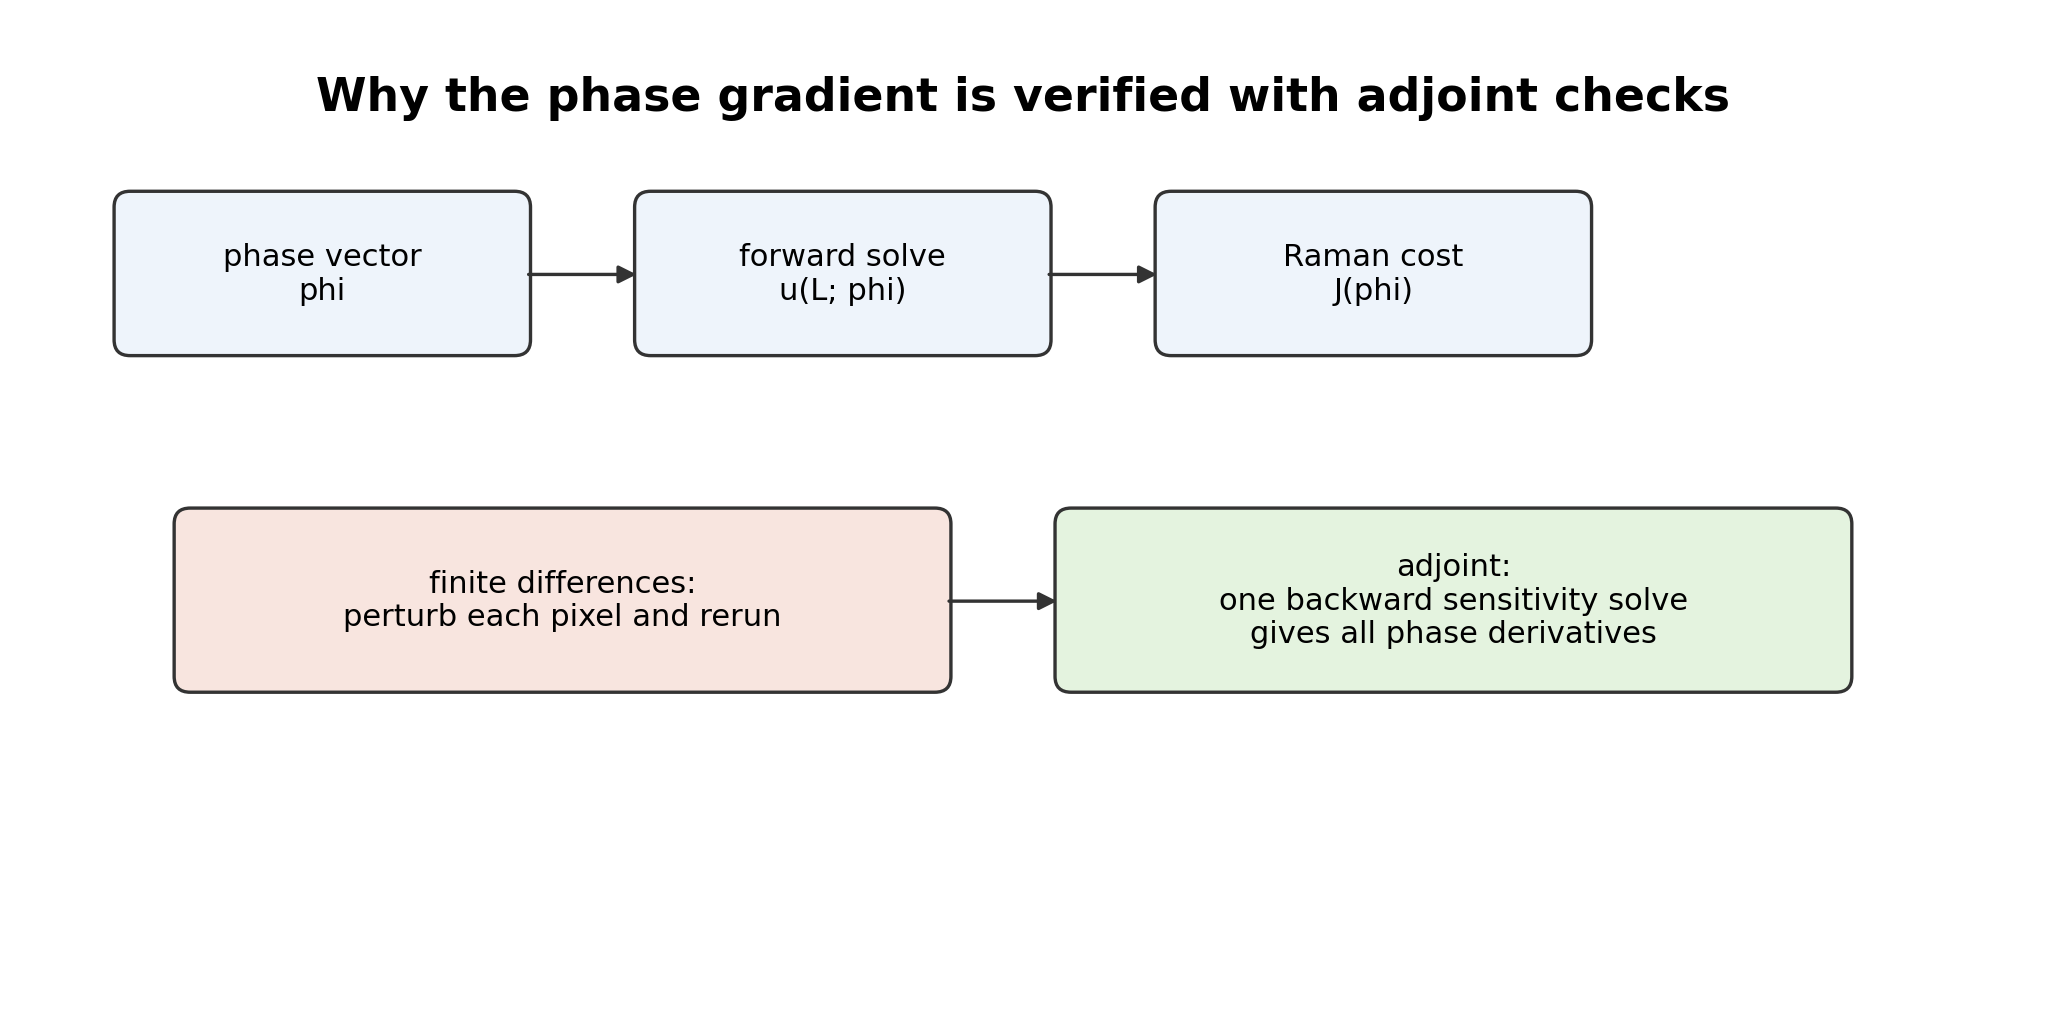
\includegraphics[width=0.92\linewidth]{figures/adjoint_gradient_check.png}
\caption{Adjoint-gradient verification logic. The adjoint replaces a
pixel-by-pixel finite-difference gradient with one backward sensitivity solve,
but it must still be checked against finite-difference or Taylor behavior.}
\end{figure}

\begin{center}
\small
\begin{tabular}{>{\raggedright\arraybackslash}p{0.30\linewidth}
                >{\raggedright\arraybackslash}p{0.58\linewidth}}
\toprule
\textbf{Implementation path} & \textbf{What to check} \\
\midrule
\shortstack[l]{\texttt{src/simulation/}\\
\texttt{sensitivity\_disp\_mmf.jl}} &
\texttt{adjoint\_disp\_mmf!} implements the backward sensitivity RHS using the
stored forward solution. \\
\shortstack[l]{\texttt{scripts/lib/}\\
\texttt{raman\_optimization.jl}} &
\texttt{cost\_and\_gradient} applies the input phase chain rule
\(2\operatorname{Re}[\lambda_0^*iu_0]\). \\
\shortstack[l]{\texttt{scripts/research/analysis/}\\
\texttt{verification.jl}} &
Taylor remainder should scale like \(O(\epsilon^2)\). \\
\bottomrule
\end{tabular}
\end{center}

\textbf{Verification status: verified with caveat.} The phase chain rule is
straightforward and the source code matches it. The full adjoint RHS is more
complex because Kerr and Raman terms contain \(u\), \(u^*\), convolution paths,
and mode tensors. The project verifies the full assembled gradient by
finite-difference/Taylor behavior rather than asking a reader to trust every
RHS subterm by inspection alone.

\subsection*{Intuition Check}

The adjoint is the ``all knobs at once'' derivative. It tells the optimizer
which phase pixels should move up or down without rerunning the fiber once per
pixel.

\section{Regularized dB Objective}

The optimizer may use a regularized linear surface
\[
    \Jlin(\phi)
    =
    \Jphys(\phi)
    +\lambda_{\mathrm{gdd}}R_{\mathrm{gdd}}(\phi)
    +\lambda_{\mathrm{edge}}R_{\mathrm{edge}}(\phi).
\]
If the run uses a dB objective, the scalar surface is
\[
    \Jsurf(\phi)=10\log_{10}\Jlin(\phi).
\]
The gradient must be scaled by the chain rule:
\[
    \nabla \Jsurf
    =
    \frac{10}{\ln 10}\frac{1}{\Jlin}\nabla \Jlin.
\]
This is an important repaired convention: regularizers are added first, and
the dB transform is applied to the full regularized scalar.

The GDD regularizer uses the second-difference stencil
\[
    R_{\mathrm{gdd}}(\phi)
    =
    \sum_{i=2}^{\Nt-1}
    \frac{(\phi_{i+1}-2\phi_i+\phi_{i-1})^2}{\Delta\omega^3}.
\]
In matrix form, if \(D_2\) is the nonperiodic second-difference matrix with row
stencil \((1,-2,1)\), then
\[
    R_{\mathrm{gdd}}(\phi)
    =
    \frac{1}{\Delta\omega^3}\|D_2\phi\|_2^2,
    \qquad
    \nabla R_{\mathrm{gdd}}
    =
    \frac{2}{\Delta\omega^3}D_2^TD_2\phi.
\]
The strict interior stencil is proportional to
\[
    \phi_{j-2}-4\phi_{j-1}+6\phi_j-4\phi_{j+1}+\phi_{j+2}.
\]
The first two and last two samples use the corresponding truncated rows from
\(D_2^TD_2\), not a periodic wraparound.

The boundary regularizer measures temporal edge fraction of the shaped input
pulse:
\[
    R_{\mathrm{edge}}(\phi)
    =
    \frac{\sum_{t_j\in \mathrm{edge}} |u(t_j,0;\phi)|^2}
         {\sum_j |u(t_j,0;\phi)|^2}.
\]
For phase-only optimization, the denominator is constant under the FFT by
Parseval's theorem because phase changes preserve spectral amplitudes. For
amplitude-enabled optimization, the denominator is not constant and the full
quotient rule is required. This is the exact distinction that the repaired
multivariable boundary-amplitude gradient checks.

\begin{center}
\small
\begin{tabular}{>{\raggedright\arraybackslash}p{0.30\linewidth}
                >{\raggedright\arraybackslash}p{0.58\linewidth}}
\toprule
\textbf{Implementation path} & \textbf{What to check} \\
\midrule
\shortstack[l]{\texttt{scripts/lib/}\\
\texttt{regularizers.jl}} &
Adds GDD and boundary regularizer scalar contributions and gradients. \\
\shortstack[l]{\texttt{scripts/lib/}\\
\texttt{objective\_surface.jl}} &
Records whether the scalar surface is linear or dB and whether regularizers
are chained into the surface. \\
numerics regression tests &
Regression coverage for the repaired objective-scale convention. \\
\bottomrule
\end{tabular}
\end{center}

\textbf{Verification status: verified.} This is the current authoritative
objective convention for single-mode phase optimization.

\subsection*{Intuition Check}

Do not compare two results unless you know what surface they optimized. A dB
objective, a linear objective, and a regularized objective can all report a
Raman number, but they did not ask the optimizer the same question.

\section{Coordinate Maps And Chain Rules}

Several research paths optimize variables that are not the raw full-grid phase.
The verification rule is always the same: map optimizer coordinates to physical
controls, then chain-rule gradients back to the optimizer coordinates.

\begin{figure}[H]
\centering
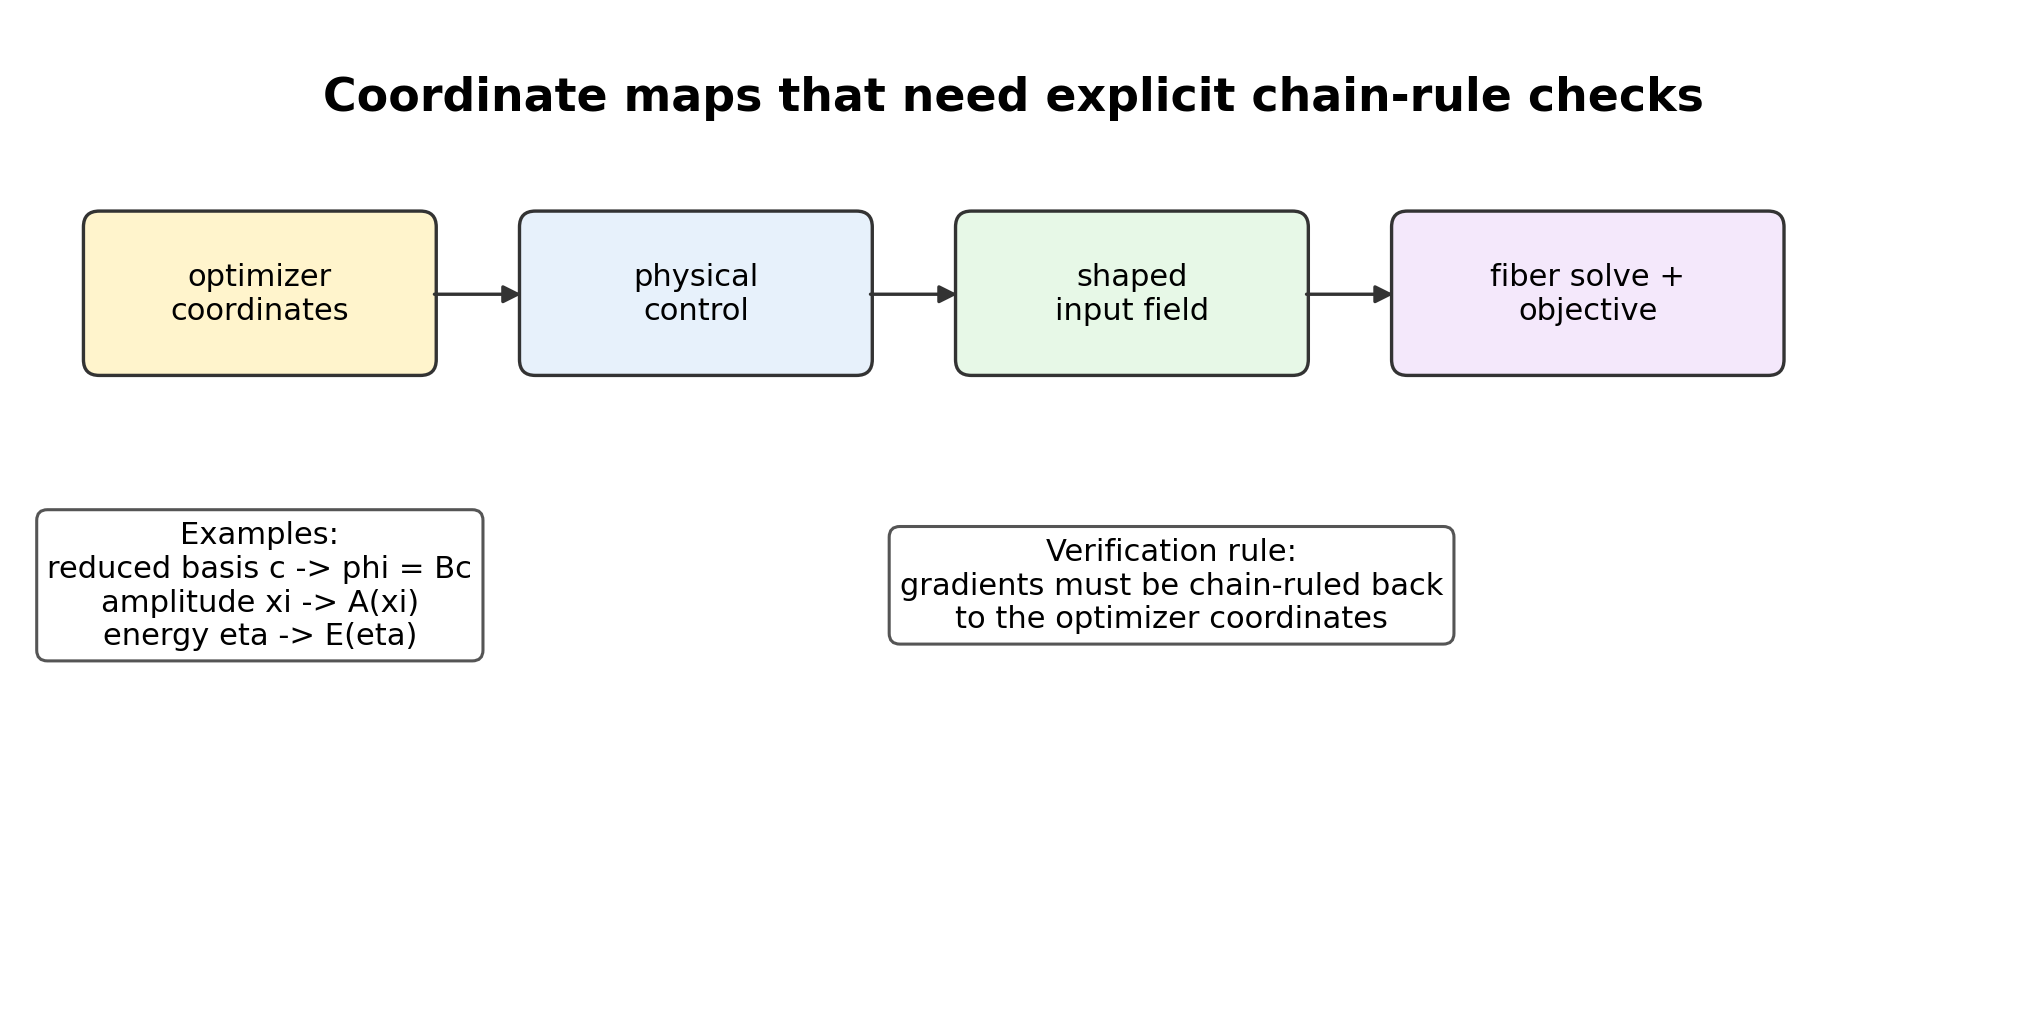
\includegraphics[width=0.92\linewidth]{figures/coordinate_chain_rules.png}
\caption{Coordinate-map verification rule. Reduced-basis, amplitude, energy,
and mode-coordinate controls all need explicit chain-rule or finite-difference
checks in the coordinates the optimizer actually uses.}
\end{figure}

\subsection{Reduced Basis}

Reduced-basis phase optimization uses
\[
    \phi = Bc,
\]
where columns of \(B\) are allowed phase shapes and \(c\) is the optimizer
coordinate vector. The gradient must satisfy
\[
    \nabla_c \Jsurf = B^T \nabla_\phi \Jsurf.
\]

\textbf{Implementation path:} reduced-basis and continuation code under
\texttt{scripts/research/phases/} plus the reduced-basis and basis-extension
regression tests.

\textbf{Verification status: verified for the active reduced-basis lane.}
The final public reduced-basis note still needs a provenance table connecting
reported numbers to saved artifacts.

\subsection{Multivariable Phase, Amplitude, And Energy}

The multivariable path can optimize phase, spectral amplitude, and scalar
energy. The same forward-adjoint sensitivity is chained through each variable.
For example, an amplitude parameterization \(A(\xi)\) needs
\[
    \frac{dJ}{d\xi}
    =
    \frac{dJ}{dA}\frac{dA}{d\xi}.
\]
The repaired boundary-amplitude gradient uses the quotient rule because edge
fraction depends on both edge energy and total input energy.

\textbf{Implementation path:}
\texttt{scripts/research/multivar/multivar\_optimization.jl}.

\textbf{Verification status: pending rerun.} A local algebra check matched
central finite differences for the repaired boundary-amplitude derivative.
The burst multivariable smoke suite still needs to be rerun before final
amplitude-enabled claims are trusted.

\section{Hessian And Trust-Region Diagnostics}

The project uses Hessian-vector products and trust-region methods as
diagnostics and candidate optimizers. The key verification point is negative:
the current HVP paths should be described as finite-difference Hessian
diagnostics unless a note explicitly proves an analytic second-adjoint path.

If \(F(\phi)=10\log_{10}\Jlin(\phi)\), then
\[
    \nabla^2F
    =
    \frac{10}{\ln 10}
    \left(
      \frac{1}{\Jlin}\nabla^2\Jlin
      -
      \frac{1}{\Jlin^2}\nabla\Jlin\nabla\Jlin^T
    \right).
\]
So a linear-cost Hessian is not automatically the Hessian of the regularized
dB optimizer surface.

\textbf{Implementation paths:}
HVP regression tests, \texttt{test/trust\_region/}, and trust-region code under
\texttt{scripts/research/trust\_region/}.

\textbf{Verification status: verified with caveat.} HVPs are useful when the
scalar surface is named. Public notes must not call them analytic Hessians
unless that is actually the path being tested.

\subsection*{Intuition Check}

Curvature depends on the surface. If we change the cost scale from linear to
dB, we changed the hill the optimizer is walking on.

\section{Multimode Derivatives}

For shared-phase multimode optimization, the phase is common across modes but
the cost depends on all propagated modal fields. The phase gradient sums the
modewise sensitivities:
\[
    \frac{dJ}{d\phi(\omega)}
    =
    \sum_m
    2\operatorname{Re}
    \left[
      \lambda_{0,m}(\omega)^*\,i\,u_{0,m}(\omega)
    \right].
\]

For phase-plus-mode-coordinate work, the mode-coordinate block is currently
finite-differenced by design. That is acceptable because the block is small
relative to the phase grid, and a previous analytic complex chain did not pass
preflight.

\textbf{Implementation paths:}

The MMF research-driver directory contains the Raman and joint-optimization
drivers. The MMF regression tests check the derivative path.

\textbf{Verification status: shared-phase verified; mode-coordinate block
finite-difference by design.} A clean burst preflight for the mode-coordinate
finite-difference block reported zero relative error in the saved summary, but
the MMF regression test should still be rerun for the final verification pass.

\section{Current Verification Matrix}

\begin{center}
\scriptsize
\resizebox{\linewidth}{!}{%
\begin{tabular}{>{\raggedright\arraybackslash}p{0.24\linewidth}
                >{\raggedright\arraybackslash}p{0.24\linewidth}
                >{\raggedright\arraybackslash}p{0.28\linewidth}
                >{\raggedright\arraybackslash}p{0.20\linewidth}}
\toprule
\textbf{Path} & \textbf{Equation status} & \textbf{Evidence} & \textbf{Public status} \\
\midrule
Forward interaction-picture GNLSE & analytic model from nonlinear fiber optics &
source audit; soliton/photon verification script exists & verified with fresh
burst rerun pending \\
Raman-band cost & quotient derivative analytic & direct cost cross-check exists &
verified, rerun pending \\
Single-mode phase gradient & analytic adjoint chain rule & Taylor and FD checks &
verified \\
GDD regularizer & analytic discrete stencil & regularized gradient tests &
verified \\
Boundary phase regularizer & analytic phase derivative & regularized gradient
tests & verified \\
Reduced basis & linear map \(\phi=Bc\) & basis tests and extension tests &
verified, provenance table still needed \\
Sharpness objective & mixed objective / robustness diagnostic & sharpness tests &
verified with scalar-surface caveats \\
HVP / trust-region & finite-difference HVP diagnostics & HVP and trust-region
tests & verified with caveat \\
MMF shared phase & analytic mode-summed chain rule & MMF FD tests & verified,
rerun pending \\
MMF mode coordinates & not analytic by current policy & finite-difference
preflight & finite-difference by design \\
Multivariable amplitude boundary term & analytic quotient-rule derivative &
local FD check & pending burst smoke rerun \\
\bottomrule
\end{tabular}}
\end{center}

\section{Required Reruns Before Final Freeze}

These should run on the burst machine through the approved heavy-job wrapper:

\begin{enumerate}
    \item \texttt{julia -t auto --project=. scripts/research/analysis/verification.jl}
    \item \texttt{julia -t auto --project=. scripts/dev/smoke/test\_multivar\_gradients.jl}
    \item Run the active MMF regression entry point from the test manifest,
    using Julia threading.
\end{enumerate}

The cost-audit missing matrix should only be rerun if the project decides that
the cost-audit note needs completed matrix coverage rather than an honest
``matrix incomplete'' status.

\section{What This Means For The Research Notes}

\textbf{Baseline and reduced-basis notes} can cite the adjoint phase-gradient,
regularized objective, and reduced-basis chain-rule sections here, but still
need result-provenance tables.

\textbf{Sharpness and trust-region notes} must name the scalar surface for every
HVP or Hessian claim.

\textbf{Multimode and multivariable notes} should remain provisional until the
specified reruns and result-regeneration decisions are complete.

\textbf{Cost/numerics note} should point here once the burst reruns are attached,
so it does not need to carry every derivation itself.

\section{Sources}

\begin{thebibliography}{9}

\bibitem{agrawal2019}
G. P. Agrawal.
\textit{Nonlinear Fiber Optics}, 6th ed.
Academic Press, 2019.
\url{https://doi.org/10.1016/C2018-0-01168-8}

\bibitem{hult2007}
J. Hult.
``A fourth-order Runge-Kutta in the interaction picture method for simulating
supercontinuum generation in optical fibers.''
\textit{Journal of Lightwave Technology}, 25(12), 3770--3775, 2007.
\url{https://doi.org/10.1109/JLT.2007.909373}

\bibitem{nocedal2006}
J. Nocedal and S. J. Wright.
\textit{Numerical Optimization}, 2nd ed.
Springer, 2006.
\url{https://doi.org/10.1007/978-0-387-40065-5}

\bibitem{frigo2005}
M. Frigo and S. G. Johnson.
``The design and implementation of FFTW3.''
\textit{Proceedings of the IEEE}, 93(2), 216--231, 2005.
\url{https://doi.org/10.1109/JPROC.2004.840301}

\end{thebibliography}

\end{document}
